\clearpage
\title{Implementing Interpolation; Newton's Backward Method in MATLAB }
\author{}
\date{}
\maketitle

\section*{Introduction}
\subsection*{Interpolation, Newton's Backward Method}
Newton's Backward Interpolation is another numerical technique used for estimating the value of a function between given data points. Similar to Newton's Forward Interpolation, it falls under the category of polynomial interpolation methods and is particularly useful for equally spaced data points.\\\\
The general form of the Newton's Backward Interpolation polynomial is:
\[f(x) = P_n(x) = f(x_n) + \Delta y_{n-1} \cdot P_1(u) + \Delta^2 y_{n-2} \cdot P_2(u) + \ldots\]
Here, \(P_n(x)\) is the polynomial of degree \(n\) used for interpolation, \(f(x_n)\) represents the value of the function at the last point \(x_n\), \(\Delta y_{n-1}\) denotes the first backward difference, \(\Delta^2 y_{n-2}\) signifies the second backward difference, and so on. The symbol \(u\) typically represents the normalized difference ratio \(\frac{x - x_n}{h}\), where \(h\) is the common difference between the data points.


\section*{Tools Used}
\begin{itemize}
    \item MATLAB R2021a - for writing and running code.
    \item MacTeX -\LaTeX  compiler.
    \item VS Code with \LaTeX workshop extension as a text editor.
\end{itemize}

\section*{Process}

\subsection*{Code for Newton's Backward Interpolation:}
\begin{minted}[breaklines, linenos]{matlab}

\end{minted}

\subsection*{Output}
\begin{center}
    \centering
    % 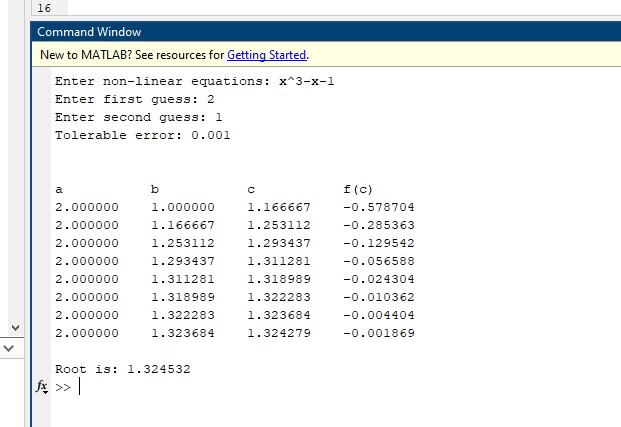
\includegraphics[width = .9\textwidth]{false.jpeg}
    \captionof{figure}{Newton's Backward Method}
\end{center}